\chapter{Discrete Random Variables}
\label{chapter:DiscreteRandomVariables}

Suppose that an experiment and a sample space are given.
A \emph{random variable} is a real-valued function of the outcome of the experiment. \index{Random variable}
In other words, the random variable assigns a specific number to every possible outcome of the experiment.
The numerical value of a particular outcome is simply called the \emph{value} of the random variable. \index{Value of a random variable}
Because of the structure of real numbers, it is possible to define pertinent statistical properties on random variables that otherwise do not apply to probability spaces in general.

\begin{figure}[ht]
\begin{center}
\begin{psfrags}
\psfrag{S}[l]{Sample Space}
\psfrag{1}[c]{$1$}
\psfrag{2}[c]{$2$}
\psfrag{3}[c]{$3$}
\psfrag{4}[c]{$4$}
\psfrag{5}[c]{$5$}
\psfrag{6}[c]{$6$}
\psfrag{7}[c]{$7$}
\psfrag{R}[r]{Real Numbers}
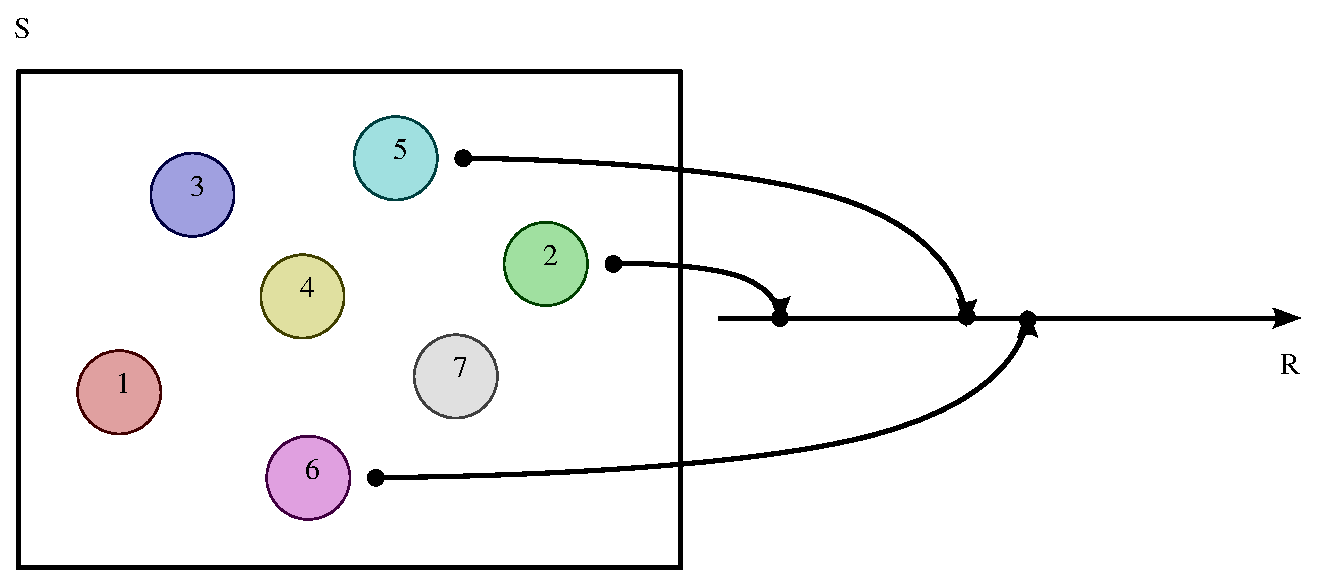
\includegraphics[height=4.96cm]{Figures/5Chapter/rv}
\caption{The sample space in this example has seven possible outcomes.
A random variable maps each of these outcomes to a real number.}
\end{psfrags}
\end{center}
\end{figure}

\begin{example}
There are six possible outcomes to the rolling of a fair die, namely each of the six faces.
These faces map naturally to the integers one through six.
The value of the random variable, in this case, is simply the number of dots that appear on the top face of the die.

\begin{figure}[ht]
\begin{center}
\begin{psfrags}
\psfrag{1}[c]{$1$}
\psfrag{2}[c]{$2$}
\psfrag{3}[c]{$3$}
\psfrag{4}[c]{$4$}
\psfrag{5}[c]{$5$}
\psfrag{6}[c]{$6$}

\includegraphics[height=5.99cm]{Figures/5chapter/rvdices}
\caption{This random variable takes its input from the rolling of a die and assigns to each outcome a real number that corresponds to the number of dots that appear on the top face of the die.}
\end{psfrags}
\end{center}
\end{figure}
\end{example}

The simplest class of random variables is the collection of \emph{discrete random variables}. \index{Discrete random variable}
A variable is called discrete if its range is finite or countably infinite; that is, if the random variable can only take a finite or countable number of values.

\begin{example}
Consider the experiment where a coin is tossed repetitively until heads is observed.
The corresponding function, which maps the number of tosses to an integer, is a discrete random variable that takes a countable number of values.
The range of this random variable is given by the positive integers $\{1, 2, \ldots \}$.
\end{example}

\section{Probability Mass Functions}

A discrete random variable $X$ is characterized by the probability of each of the elements in the range of $X$.
We identify the probabilities of individual elements in the range of $X$ using the \emph{probability mass function (PMF)} of $X$, which we denote by $p_X$. \index{Probability mass function (PMF)}
If $x$ is a possible value of $X$ then the \emph{probability mass} of $x$, written $p_X (x)$, is defined by
\begin{equation} \label{equation:PMF}
p_X (x) = \Pr ( \{ X = x \} ) = \Pr ( X = x ) .
\end{equation}
Equivalently, we can think of $p_X (x)$ as the probability of the set of all outcomes in $\Omega$ for which $X$ is equal to $x$,
\begin{equation*}
p_X (x)
= \Pr (  X^{-1} (x)  )
= \Pr ( \{ \omega \in \Omega | X(\omega) = x \} ) .
\end{equation*}

\begin{figure}[ht]
\begin{center}
\begin{psfrags}
\psfrag{S}[l]{Sample Space}
\psfrag{1}[c]{$1$}
\psfrag{2}[c]{$2$}
\psfrag{3}[c]{$3$}
\psfrag{4}[c]{$4$}
\psfrag{5}[c]{$5$}
\psfrag{6}[c]{$6$}
\psfrag{7}[c]{$7$}
\psfrag{x}[l]{$x$}
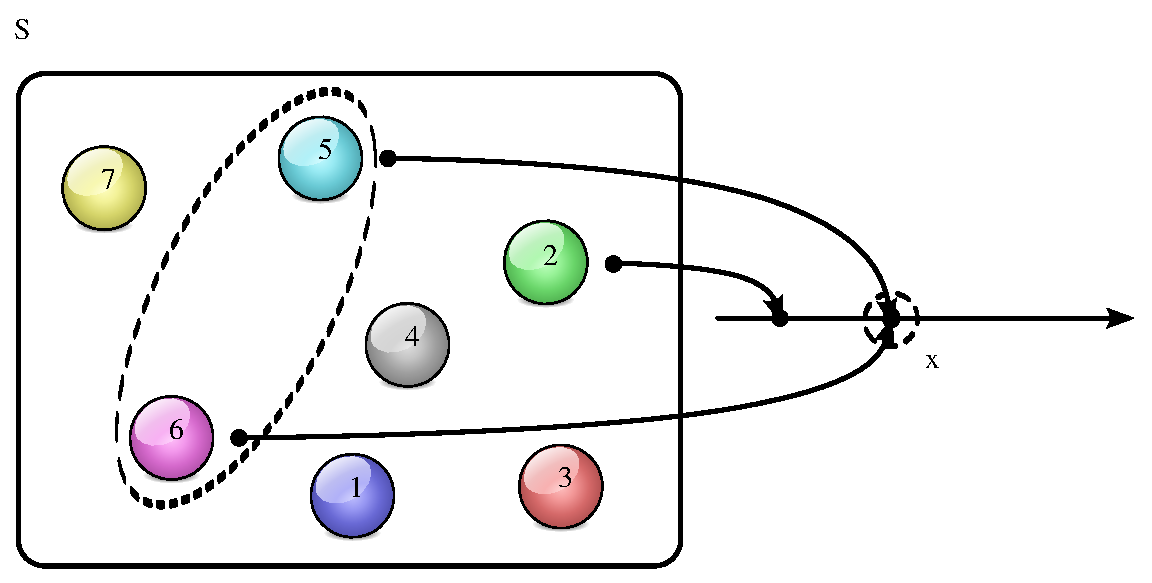
\includegraphics[height=4.97cm]{Figures/5Chapter/pmf}
\caption{The probability mass of $x$ is given by the probability of the set of all outcomes which $X$ maps to $x$.}
\end{psfrags}
\end{center}
\end{figure}


Let $X(\Omega)$ denote the collection of all the possible numerical values $X$ can take; this set is known as the range of $X$.
Using this notation, we can write
\begin{equation} \label{equation:NormalizationPMF}
\sum_{x \in X(\Omega)} p_X(x) = 1 .
\end{equation}
We emphasize that the sets defined by $\{ \omega \in \Omega | X(\omega) = x \}$ are disjoint and form a partition of the sample space $\Omega$, as $x$ ranges over all the possible values in $X (\Omega)$.
Thus, \eqref{equation:NormalizationPMF} follows immediately from the countable additivity axiom and the normalization axiom of probability laws.
In general, if $X$ is a discrete random variable and $S$ is a subset of $X(\Omega)$, we can write
\begin{equation} \label{equation:FunctionPMF}
\Pr (S) = \Pr \left( \{ \omega \in \Omega | X(\omega) \in S \} \right) = \sum_{x \in S} p_X (x) .
\end{equation}
This equation offers an explicit formula to compute the probability of any subset of $X (\Omega)$, provided that $X$ is discrete.

\begin{example}
An urn contains three balls numbered one, two and three.
Two balls are drawn from the urn without replacement.
We wish to find the probability that the sum of the two selected numbers is odd.

Let $\Omega$ be the set of ordered pairs corresponding to the possible outcomes of the experiment,
$\Omega = \{ (1, 2), (1, 3), (2, 1), (2, 3), (3, 1), (3, 2) \}$.
Note that these outcomes are equiprobable.
We employ $X$ to represent the sum of the two selected numbers.
The PMF of random variable $X$ is given by
\begin{equation*}
p_X (3) = p_X (4) = p_X (5) = \frac{1}{3}.
\end{equation*}
If $S$ denotes the event that the sum of the two numbers is odd, then the probability of the sum being odd can be computed as follows,
\begin{equation*}
\Pr (S) = \Pr ( \{ 3, 5 \} )
= p_X (3) + p_X (5) = \frac{2}{3} .
\end{equation*}
\end{example}


\section{Important Discrete Random Variables}

A number of discrete random variables appears frequently in problems related to probability.
These random variables arise in many different contexts, and they are worth getting acquainted with.
In general, discrete random variables occur primarily in situations where counting is involved.


\subsection{Bernoulli Random Variables}

The first and simplest discrete random variable is the \emph{Bernoulli random variable}. \index{Bernoulli random variable}
Let $X$ be a random variable that takes on only two possible numerical values, $X(\Omega) = \{0, 1\}$.
Then $X$ is a Bernoulli random variable and its PMF is given by
\begin{equation*}
p_X (x) = \left\{ \begin{array}{ll}
1 - p, & \text{if }x = 0 \\
p, & \text{if }x = 1
\end{array} \right.
\end{equation*}
where $p \in [0, 1]$.

\begin{figure}[ht]
\begin{center}
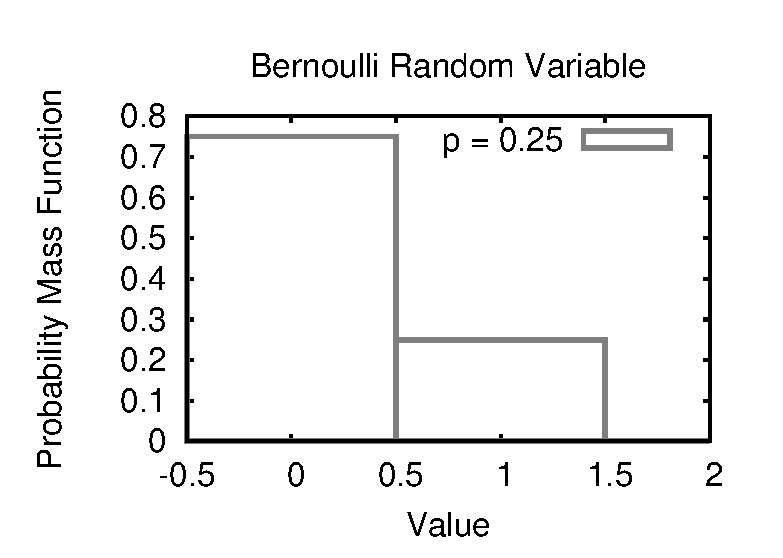
\includegraphics[width=8.5cm]{Figures/5chapter/bernoulli_pmf}
\end{center}
\caption{The PMF of a Bernoulli random variable appears above for parameter $p = 0.25$.}
\end{figure}

\begin{example}
Consider the flipping of a biased coin, for which heads is obtained with probability $p$ and tails is obtained with probability $1-p$.
A random variable that maps heads to one and tails to zero is a Bernoulli random variable with parameter~$p$.
In fact, every Bernoulli random variable is equivalent to the tossing of a coin.
\end{example}


\subsection{Binomial Random Variables}
\label{subsection:BinormialRandomVariables}

Multiple independent Bernoulli random variables can be combined to construct more sophisticated random variables.
Suppose $X$ is the sum of $n$ independent and identically distributed Bernoulli random variables.
Then $X$ is called a \emph{binomial random variable} with parameters $n$ and $p$. \index{Binomial random variable}
The PMF of $X$ is given by
\begin{equation*}
p_X (k) = \Pr (X = k)
= \binom{n}{k} p^k (1-p)^{n-k},
\end{equation*}
where $k = 0, 1, \ldots n$.
Note that we can easily verify that $X$ fulfills the normalization axiom,
\begin{equation*}
\sum_{k=0}^n \binom{n}{k} p^k (1-p)^{n-k}
= \left( p + (1-p) \right)^n = 1.
\end{equation*}

\begin{figure}[ht]
\begin{center}
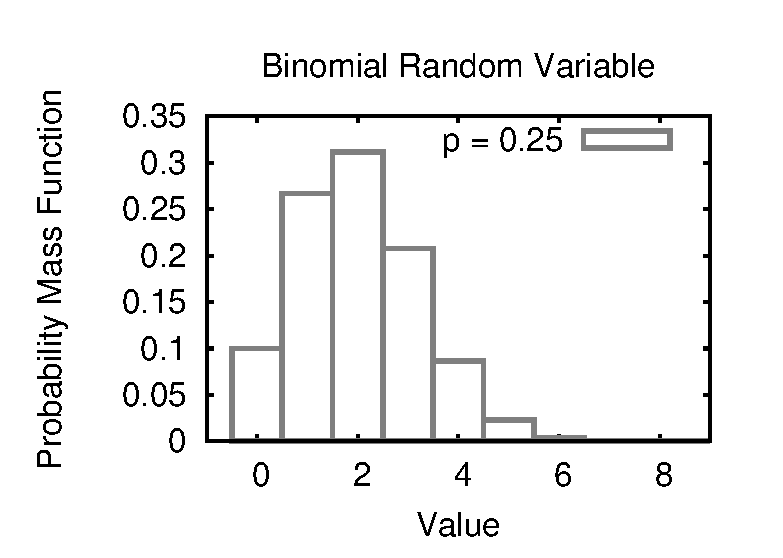
\includegraphics[width=8.5cm]{Figures/5chapter/binomial_pmf}
\end{center}
\caption{This figure shows a binomial random variable with parameters $n = 8$ and $p = 0.25$.}
\end{figure}

\begin{example} \label{BrazosSodaCompany1}
The Brazos Soda Company creates an ``Under the Caps'' promotion whereby a customer can win an instant cash prize of \$1 by looking under a bottle cap.
The likelihood to win is one in four, and it is independent from bottle to bottle.
A customer buys eight bottles of soda from this company.
We wish to find the PMF of the number of winning bottles, which we denote by $X$.
Also, we want to compute the probability of winning more than \$4.

The random variable $X$ is binomial with parameters $n = 8$ and $p = 1/4$.
Its PMF is given by
\begin{equation*}
p_X (k) = \binom{8}{k} \left( \frac{1}{4} \right)^k
\left( \frac{3}{4} \right)^{8-k}
= \binom{8}{k} \frac{3^{8-k}}{4^8} ,
\end{equation*}
where $k = 0, 1, \ldots, 8$.
The probability of winning more than \$4 is
\begin{equation*}
\Pr ( X\$ > \$4)
= \Pr (X > 4)
= \sum_{k=5}^{8} \binom{8}{k} \frac{3^{8-k}}{4^8} .
\end{equation*}
\end{example}


\subsection{Poisson Random Variables}

The probability mass function of a \emph{Poisson random variable} is given by \index{Poisson random variable}
\begin{equation*}
p_X (k) = \frac{\lambda^k}{k!} e^{- \lambda}, \quad k = 0, 1, \ldots
\end{equation*}
where $\lambda$ is a positive number.
Note that, using Taylor series expansion,  we have
\begin{equation*}
\sum_{k = 0}^{\infty} p_X (k)
= \sum_{k = 0}^{\infty} \frac{\lambda^k}{k!} e^{- \lambda}
= e^{- \lambda} \sum_{k = 0}^{\infty} \frac{\lambda^k}{k!}
= e^{- \lambda} e^{\lambda} = 1 ,
\end{equation*}
which shows that this PMF fulfills the normalization axiom of probability laws.
The Poisson random variable is of fundamental importance when counting the number of occurrences of a phenomenon in a certain time period.
It finds extensive use in networking, inventory management and queueing applications.

\begin{figure}[ht]
\begin{center}
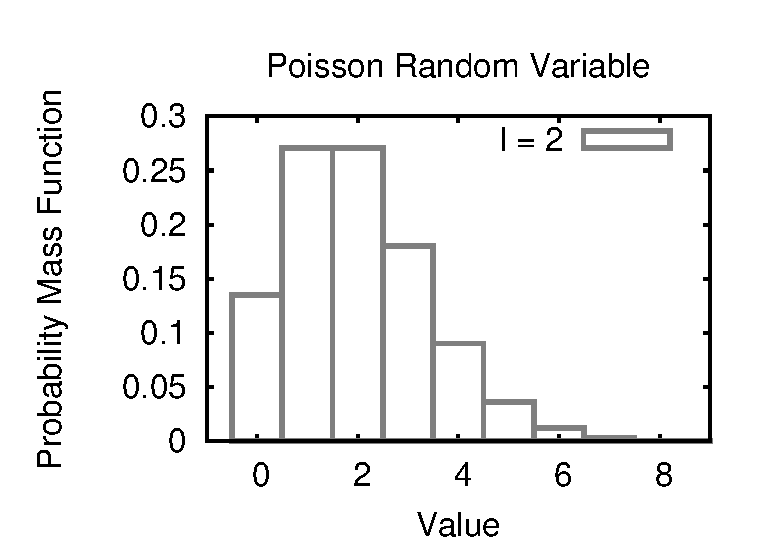
\includegraphics[width=8.5cm]{Figures/5chapter/poisson_pmf}
\caption{This figure shows the PMF of a Poisson random variable with parameter $\lambda = 2$.  Note that the values of the PMF are only present for $k = 0, 1, \ldots, 8$.}
\end{center}
\end{figure}

\begin{example}
Requests at an Internet server arrive at a rate of $\lambda$ connections per second.
The number of service requests per second is modeled as a random variable with a Poisson distribution.
We wish to find the probability that no service requests arrive during a time interval of one second.

Let $N$ be a random variable that represents the number of requests that arrives within a span of one second.
By assumption, $N$ is a Poisson random variable with PMF
\begin{equation*}
p_N (k) = \frac{ \lambda^k }{k!} e^{-\lambda} .
\end{equation*}
The probability that no service requests arrive in one second is simply given by $p_N (0) = e^{-\lambda}$.
\end{example}

It is possible to obtain a Poisson random variable as the limit of a sequence of binomial random variables.
Fix $\lambda$ and let $p_n = \lambda/n$.
For $k = 1, 2, \ldots n$, we define the PMF of the random variable $X_n$ as
\begin{equation*}
\begin{split}
p_{X_n} (k) &= \Pr (X_n = k)
= \binom{n}{k} p_n^k (1-p_n)^{n-k} \\
&= \frac{n!}{k!(n-k)!} \left( \frac{\lambda}{n} \right)^k
\left( 1 - \frac{\lambda}{n} \right)^{n-k} \\
&= \frac{n!}{n^k (n-k)!} \frac{\lambda^k}{k!}
\left( 1 - \frac{\lambda}{n} \right)^{n-k} .
\end{split}
\end{equation*}
In the limit, as $n$ approaches infinity, we get
\begin{equation*}
\lim_{n \rightarrow \infty} p_{X_n} (k)
= \lim_{n \rightarrow \infty} \frac{n!}{n^k (n-k)!} \frac{\lambda^k}{k!}
\left( 1 - \frac{\lambda}{n} \right)^{n-k}
= \frac{\lambda^k}{k!} e^{- \lambda} .
\end{equation*}
Thus, the sequence of binomial random variables $\{ X_n \}$ converges in distribution to the Poisson random variable $X$.

\begin{figure}[ht]
\begin{center}
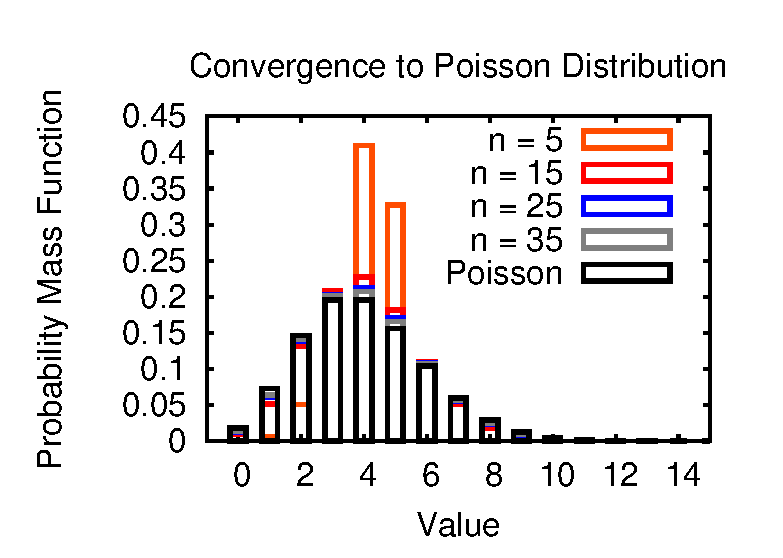
\includegraphics[width=8.5cm]{Figures/5chapter/convergence_pmf}
\end{center}
\caption{The levels of a binomial PMF with parameter $p = \lambda/n$ converge to the probabilities of a Poisson PMF with parameter $\lambda$ as $n$ increases to infinity.}
\end{figure}

This discussion suggests that the Poisson PMF can be employed to approximate the PMF of a binomial random variable in certain circumstances.
Suppose that $Y$ is a binomial random variable with parameters $n$ and $p$.
If $n$ is large and $p$ is small then the probability that $Y$ equals $k$ can be approximated by
\begin{equation*}
p_{Y} (k) = \frac{n!}{n^k (n-k)!} \frac{\lambda^k}{k!}
\left( 1 - \frac{\lambda}{n} \right)^{n-k}
\approx \frac{\lambda^k}{k!} e^{- \lambda} ,
\end{equation*}
where $\lambda = n p$.
The latter expression can be computed numerically in a straightforward manner.

\begin{example}
The probability of a bit error on a wireless communication channel is equal to $10^{-2}$.
We wish to approximate the probability that a block of $1000$ bits has four or more errors.

Assume that the probability of individual errors is independent from bit to bit.
The transmission of each bit can be modeled as a Bernoulli trial, with a zero indicating a correct transmission and a one representing a bit error.
The total number of bit errors in $1000$ transmissions then corresponds to a binomial random variable with parameters $n = 1000$ and $p = 10^{-2}$.
The probability of making four or more errors can be approximated using a Poisson random variable with constant $\lambda = np = 10$.
Thus, we can approximate the probability that a block of $1000$ bits has four or more errors by
\begin{equation*}
\begin{split}
\Pr [ N \geq 4 ] &= 1 - \Pr [ N < 4 ]
\approx 1 - \sum_{k=0}^3 \frac{\lambda^k}{k!} e^{-\lambda} \\
&= 1 - e^{-10} \left( 1 + 10 + 50 + \frac{500}{3} \right) \\
&\approx 0.01034 .
\end{split}
\end{equation*}
% The exact value in this case is
\end{example}


\subsection{Geometric Random Variables}

Consider a random experiment where a Bernoulli trial is repeated multiple times until a one is observed.
At each time step, the probability of getting a one is equal to $p$ and the probability of getting a zero is $1-p$.
The number of trials carried out before completion, which we denote by $X$, is recorded as the outcome of the experiment.
The random variable $X$ is a \emph{geometric random variable}, and its PMF is given by \index{Geometric random variable}
\begin{equation*}
p_X (k) = (1-p)^{k-1} p, \quad k = 1, 2, \ldots
\end{equation*}
We stress that $(1-p)^{k-1} p$ simply represents the probability of obtaining a sequence of $k-1$ zero immediately followed by a one.

\begin{figure}[ht]
\begin{center}
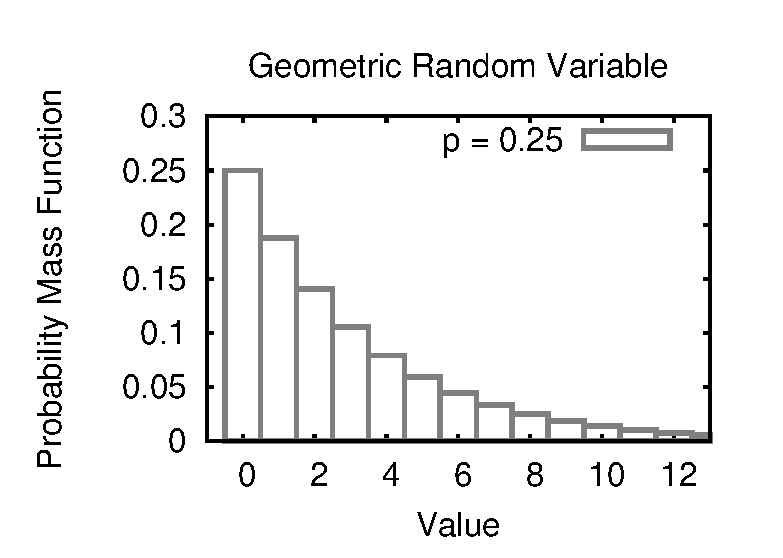
\includegraphics[width=8.5cm]{Figures/5chapter/geometric_pmf}
\end{center}
\caption{The PMF of a geometric random variable is a decreasing function of $k$.
It is plotted above for $p = 0.25$.
The values of the PMF are only present for $k = 1, 2, \ldots, 12$.}
\end{figure}

\begin{example}
The Brazos Soda Company introduces another ``Under the Caps'' promotion.
This time, a customer can win an additional bottle of soda by looking under the cap of her bottle.
The probability to win is $1/5$, and it is independent from bottle to bottle.
A customer purchases one bottle of soda from the Brazos Soda company and hence enters the contest.
For every extra bottle of soda won by looking under the cap, the customer gets an additional chance to play.
We wish to find the PMF of the number of bottles obtained by this customer.

Let $X$ denote the total number of bottles obtained by this customer.
The random variable $X$ is geometric and its PMF is
\begin{equation*}
p_X (k) = \left( \frac{1}{5} \right)^{k-1} \frac{4}{5},
\end{equation*}
where $k = 1, 2, \ldots$
\end{example}

\paragraph{Memoryless Property:}
A remarkable aspect of the geometric random variable is that it satisfies the \emph{memoryless property}, \index{Memoryless property}
\begin{equation*}
\Pr (X = k + j | X > k) = \Pr (X = j).
\end{equation*}
This can be established using the definition of conditional probability.
Let $X$ be a geometric random variable with parameter $p$, and assume that $k$ and $j$ are positive integers.
We can write the conditional probability of $X$ as
\begin{equation*}
\begin{split}
\Pr (X = k + j | X > k)
&= \frac{\Pr( \{ X =  k + j \} \cap \{ X > k \} ) }{ \Pr ( X > k ) } \\
&= \frac{\Pr( X = k + j ) }{ \Pr ( X > k ) }
= \frac{(1 - p)^{k + j - 1} p }{ (1 - p)^k  } \\
&= (1 - p)^{j - 1} p
= \Pr (X = j).
\end{split}
\end{equation*}
In words, the probability that the number of trials carried out before completion is $k + j$, given $k$ unsuccessful trials, is equal to the unconditioned probability that the total number of trials is $j$.
It can be shown that the geometric random variable is the only discrete random variable that possesses the memoryless property.


\subsection{Discrete Uniform Random Variables}

A finite random variable where all the possible outcomes are equally likely is called a \emph{discrete uniform random variable}. \index{Uniform random variable (discrete)}
Let $X$ be a uniform random variable taking value in $X (\Omega) = \{ 1, 2, \ldots, n \}$.
Its PMF is therefore given by
\begin{equation*}
p_X (k) = \left\{ \begin{array}{ll}
1/n, & \text{if }k = 1, 2, \ldots, n \\
0, & \text{otherwise} .
\end{array} \right.
\end{equation*}
We encountered specific cases of this random variable before.
The tossing of a fair coin and the rolling of a die can both be used to construct uniform random variables.

\begin{figure}[ht]
\begin{center}
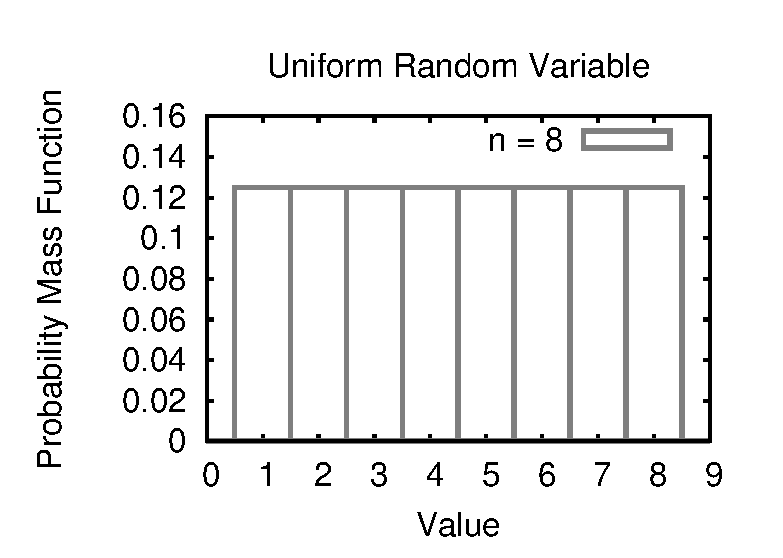
\includegraphics[width=8.5cm]{Figures/5chapter/uniform_pmf}
\end{center}
\caption{A uniform random variable corresponds to a situation where all the possible values of the random variable are equally likely.
It is shown above for the case where $n = 8$.}
\end{figure}


\section{Functions of Random Variables}
\label{subsection:FunctionDiscreteRV}
\index{Functions of Random Variables}

Recall that a random variable is a function of the outcome of an experiment.
Given a random variable $X$, it is possible to create a new random variable $Y$ by applying a real-valued function $g(\cdot)$ to $X$.
If $X$ is a random variable then $Y = g(X)$ is also a random variable since it associates a numerical value to every outcome of the experiment.
In particular, if $\omega \in \Omega$ is the outcome of the experiment, then $X$ takes on value $x = X(\omega)$ and $Y$ takes on value $Y(\omega) = g(x)$.

\begin{figure}[htb!]
\begin{center}
\begin{psfrags}
\psfrag{1}[c]{$1$}
\psfrag{2}[c]{$2$}
\psfrag{3}[c]{$3$}
\psfrag{4}[c]{$4$}
\psfrag{5}[c]{$5$}
\psfrag{S}[l]{Sample Space}
\psfrag{X}[c]{$X$}
\psfrag{Y}[c]{$Y = g(X)$}
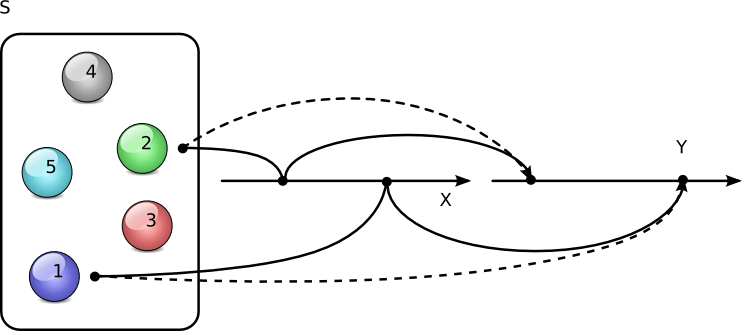
\includegraphics[height=4.97cm]{Figures/5Chapter/fcn}
\end{psfrags}
\caption{A real-valued function of a random variable is a random variable itself.
In this figure, $Y$ is obtained by passing random variable $X$ through a function $g$.}
\end{center}
\end{figure}

Furthermore, if $X$ is a discrete random variable, then so is $Y$.
The set of all the possible values $Y$ can take is denoted by $g(X(\Omega))$, and the number of elements in $g(X(\Omega))$ is no greater than the number of elements in $X(\Omega)$.
The PMF of $Y$, which we represent by $p_Y (y)$, is obtained as follows.
If $y \in g(X(\Omega))$ then
\begin{equation} \label{equation:DefinitionFunctionPMF}
p_Y (y) = \sum_{ \{x \in X(\Omega) | g(x) = y \} } p_X (x) ;
\end{equation}
otherwise, $p_Y (y) = 0$.
In particular, $p_Y (y)$ is non-zero only if there exists an $x \in X(\Omega)$ such that $g(x) = y$ and $p_X (x) > 0$.

\begin{example}
Let $X$ be a random variable and let $Y = g(X) = aX + b$, where $a$ and $b$ are constant.
That is, $Y$ is an affine function of $X$.
Suppose that $a \neq 0$, then the probability of $Y$ being equal to value $y$ is given by
\begin{equation*}
p_Y(y) = p_X \left( \frac{ y - b }{a} \right) .
\end{equation*}
\end{example}

Linear and affine functions of random variables are commonplace in probability.
In Example~\ref{BrazosSodaCompany1}, for instance, we have implicitly used the linear function $Y = 10 X$ to compute the probability of winning more than \$40.


\section*{Further Reading}

\begin{small}
\begin{enumerate}
\item Ross, S., \emph{A First Course in Probability}, 7th edition, Pearson Prentice Hall,2006: Sections~4.1--4.2, 4.6--4.8.
\item Bertsekas, D.P., and Tsitsiklis, J.N., \emph{Introduction to Probability}, Athena Scientific, 2002: Sections~2.1--2.3.
\end{enumerate}
\end{small}

